%% Copyright (C) 2008 Johan Oudinet <oudinet@lri.fr>
%%
%% Permission is granted to make and distribute verbatim copies of
%% this manual provided the copyright notice and this permission notice
%% are preserved on all copies.
%%
%% Permission is granted to process this file through TeX and print the
%% results, provided the printed document carries copying permission
%% notice identical to this one except for the removal of this paragraph
%% (this paragraph not being relevant to the printed manual).
%%
%% Permission is granted to copy and distribute modified versions of this
%% manual under the conditions for verbatim copying, provided that the
%% entire resulting derived work is distributed under the terms of a
%% permission notice identical to this one.
%%
%% Permission is granted to copy and distribute translations of this manual
%% into another language, under the above conditions for modified versions,
%% except that this permission notice may be stated in a translation
%% approved by the Free Software Foundation
%%
\chapter{Presentation of the context of the task}
\label{sec:intro}
In this chapter, several brief presentations will be given to explain the context of the human pose estimation and describe the COCO dataset.

\section{Human Pose Estimation}
\label{sec:isauriam}
Localizing body parts for human body is a fundamental yet challenging task in computer vision, and it serves as an important basis for high-level vision tasks, e.g., activity
recognition\cite{yang2010recognizing, wang2013approach}, human re-identification\cite{zheng2017pose}, and human-computer interaction.
In general,a human pose estimation model aims to predict the 2D coordinates of different human parts given a 2D human image.
Achieving accurate localization, however, is difficult due to the highly articulated human body limbs, occlusion, change of viewpoint, and foreshortening.

Classical approaches tackling the problem of human pose estimation mainly adopt the techniques of pictorial structures \cite{fischler1973representation} or graphical models\cite{chen2014articulated}.
More specifically, the classical works\cite{andriluka2009pictorial, gkioxari2013articulated, sapp2013modec, johnson2011learning} formulate the problem of human keypoints estimation as a tree-structured or graphical model problem and predict keypoint locations based on hand-crafted features.
Recent works\cite{newell2016stacked, gkioxari2016chained, wei2016convolutional, insafutdinov2016deepercut} mostly rely on the development of convolutional neural network(CNN)\cite{lecun1998gradient, he2016deep}, which largely improve the performance of pose estimation.
And the rest of report also focuses on the solution based on CNN.

Nowadays there exists two main topics in human pose estimation: single person pose estimation and multi-person pose estimation. Obviously, multi-person is more challenging than single person pose estimaion but single person is the fundamentation for multi-person pose estimation, as shown in Figure.1.

\captionsetup[figure]{labelformat=empty}
\begin{figure}
  \centering
  \subfigure[Single person pose estimation]{
    \label{fig:subfig:a} %% label for first subfigure
    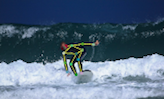
\includegraphics[width=5cm,height=4cm]{source/single.png}}
  \hspace{1in}
  \subfigure[Multi-person pose estimation]{
    \label{fig:subfig:b} %% label for second subfigure
    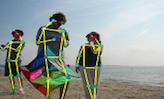
\includegraphics[width=5cm,height=4cm]{source/multi.png}}
  \caption{Figure 1:(a) is the example of single person pose estimation, only one person in a image. (b) is the example of multi-persion pose
  estimation. An image includes several peoples. We need to detect all the keypoints and group them into the right person ID.}
  \label{fig:1} %% label for entire figure
\end{figure}

\subsection{Single person Pose Estimation}
The works based on CNN usually adopts two methods: regress the coordinates of keypoints directly and regress the cofidence score map of keypoints. Toshev \textit{et al.} firstly introduce
CNN to solve pose estimation problem in the work of DeepPose\cite{toshev2014deeppose}, which proposes a cascade of CNN keypoint coordinate regressors to deal with pose estimation. Tompson \textit{et al.}\cite{tompson2014joint}
attempt to solve the problem by predicting heatmaps of keypoints using CNN and graphical models.
Using heatmap as the supervised label can provide more robust information, hence recently most of work focus on predicting heatmaps.
For example, latest works such as Wei \textit{et al.}\cite{wei2016convolutional} and Newell \textit{et al.}\cite{newell2016stacked} show great performance via generating the score map of keypoints using very
deep convolutional neural networks.

\subsection{Multi-person Pose estimation}
Multi-person pose estimation is gaining increasing popularity recently because of the high demand for the real-life applications.
However, multi-person pose estimation is challenging owing to occlusion, various gestures of individual persons and unpredictable interactions between different persons.
The approach of multi-person pose estimation is mainly divided into two categories: bottom-up approaches and top-down approaches.

\subsubsection{Bottom-Up Approaches}

Bottom-up approaches\cite{newell2017associative, insafutdinov2016deepercut, pishchulin2016deepcut} directly predict all keypoints at first and assemble them into full poses of all persons.
DeepCut\cite{pishchulin2016deepcut} interprets the problem of distinguishing different persons in an image as an Integer Linear Program (ILP) problem and partition
part detection candidates into person clusters.
Then the final pose estimation results are obtained when person clusters are combined with labeled body parts.
DeeperCut\cite{insafutdinov2016deepercut} improves DeepCut\cite{pishchulin2016deepcut} using deeper ResNet\cite{he2016deep} and employs image-conditioned pairwise terms to get better performance.
Zhe Cao \textit{et al.}\cite{cao2016realtime} map the relationship between keypoints into part affinity fields (PAFs) and assemble detected keypoints into different poses of people.
Newell \textit{et al.}\cite{newell2017associative} simultaneously produce score maps and pixel-wise embedding to group the candidate keypoints to different people to get final multi-person pose estimation.

\subsubsection{Top-down Approaches}
Top-down approaches\cite{huang2017coarse, papandreou2017towards, he2017mask} interpret the process of detecting keypoints as a twostage pipeline, that is, firstly locate and crop all persons from image,
and then solve the single person pose estimation problem in the cropped person patches.
Papandreou \textit{et al.}\cite{papandreou2017towards} predict both heatmaps and offsets of the points on the heatmaps to the ground truth location, and then uses the heatmaps with offsets to obtain the final predicted location of keypoints.
Mask-RCNN\cite{he2017mask} predicts human bounding boxes first and then crops the feature map of the corresponding human bounding box to predict human keypoints.
If top-down approach is utilized for multi-person pose estimation, a human detector as well as single person pose estimator is important in order to obtain a good performance.

\subsubsection{Human detection}
Human detection approaches are mainly guided by the RCNN family\cite{girshick2014rich, girshick2015fast, ren2015faster}, the upto-date detectors of which are\cite{lin2017feature, he2017mask}.
These detection approaches are composed of two-stage in general.
First generate boxes proposals based on default anchors, and then crop from the feature map and further refine the proposals to get the final boxes via R-CNN network.


\section{COCO dataset and metric}

COCO\cite{lin2014microsoft} is a large-scale object detection, segmentation, and captioning dataset\footnote{More details about COCO dataset can be found in http://cocodataset.org/}.
For different tasks like object detection, keypoint detection, stuff segmentaion, etc, COCO dataset can be seperated as different sub-datasets.
Here we only introduce the human keypoint dataset.

\subsection{Annotation format}

Each person(instance) annotations contains a series of fields. \textbf{1.} image\_id: Indicates which images this person belongs to. \textbf{2.} bbox: Indicates the location of this person in the image.
\textbf{3.} keypoints: a is a length 3*17 array, indicates the details of the keypoints. Each keypoint has a 0-indexed location x,y and a visibility flag v defined as v=0: not labeled (in which case x=y=0), v=1: labeled but not visible, and v=2: labeled and visible.

There are 17 keypoints: 0: nose, 1: left eye, 2: right eye, 3: left ear, 4: right ear, 5: left shoulder, 6: right shoulder, 7: left elbow, 8: right elbow, 9: left wrist, 10: right wrist, 11: left hip, 12: right hip, 13: left knee, 14: right knee, 15: left ankle, 16: right ankle.

\begin{lstlisting}
int a  = b;
\end{lstlisting}


%%% Local Variables:
%%% mode: latex
%%% TeX-master: "rapportM2R"
%%% End:
